\documentclass{standalone}
\usepackage{tikz}
\usetikzlibrary{automata, positioning, arrows}

\begin{document}
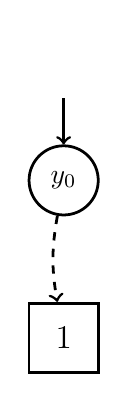
\begin{tikzpicture}[auto,node distance=1.5cm,every node/.style={shape=circle , align=center,solid,minimum size =0.01cm},line width =1pt]
  \tikzstyle{every state}=[fill=white,draw=black,text=black]

  \node[state] (B) {$y_0$};
  \node[state,shape = rectangle] (H) at ([shift = ({-90:2cm})]B) {\large$1$};
  \node[state,draw=none] (I) [above of= B]       {};

  \path[->]
  (B) edge[bend right=10,dashed]  node {} (H)
  (I) edge node{} (B);

\end{tikzpicture}
\end{document}